\documentclass[11pt, a4paper]{article}
\usepackage{geometry}
\geometry{top=1in,left=1in}
\usepackage{placeins}
\usepackage{amsmath}
\usepackage{graphicx}
\usepackage[square,numbers,sort&compress]{natbib}
\usepackage{resizegather}
\usepackage{xcolor}
\usepackage{siunitx} 
\usepackage[colorlinks=true,allcolors=blue]{hyperref}

\begin{document}

\title{Solution to the anthill problem}
\date{25th April 2024}
\author{Guru Sreevanshu Yerragolam}
\maketitle

\section{Problem Statement}

An ant leaves its anthill in order to forage for food. It moves with the speed of \SI{10}{cm/s}, but it doesn't know where to go, therefore every second it moves randomly \SI{10}{cm} directly north, south, east or west with equal probability.

\begin{enumerate}
    \item If the food is located on east-west lines \SI{20}{cm} to the north and \SI{20}{cm} to the south, as well as on north-south lines \SI{20}{cm} to the east and \SI{20}{cm} to the west from the anthill, how long will it take the ant to reach it on average?
    \item What is the average time the ant will reach food if it is located only on a diagonal line passing through $(\SI{10}{cm}, \SI{0}{cm})$ and $(\SI{0}{cm}, \SI{10}{cm})$ points?
    \item Can you write a program that comes up with an estimate of average time to find food for any closed boundary around the anthill? What would be the answer if food is located outside an area defined by $\left( (x - \SI{2.5}{cm}) / \SI{30}{cm} \right)^2 + \left( (y - \SI{2.5}{cm}) / \SI{40}{cm} \right)^2 < 1$ in coordinate system where the anthill is located at $(x = \SI{0}{cm}, y = \SI{0}{cm})$?
\end{enumerate}

\section{Analytical Solution}

\begin{figure}
    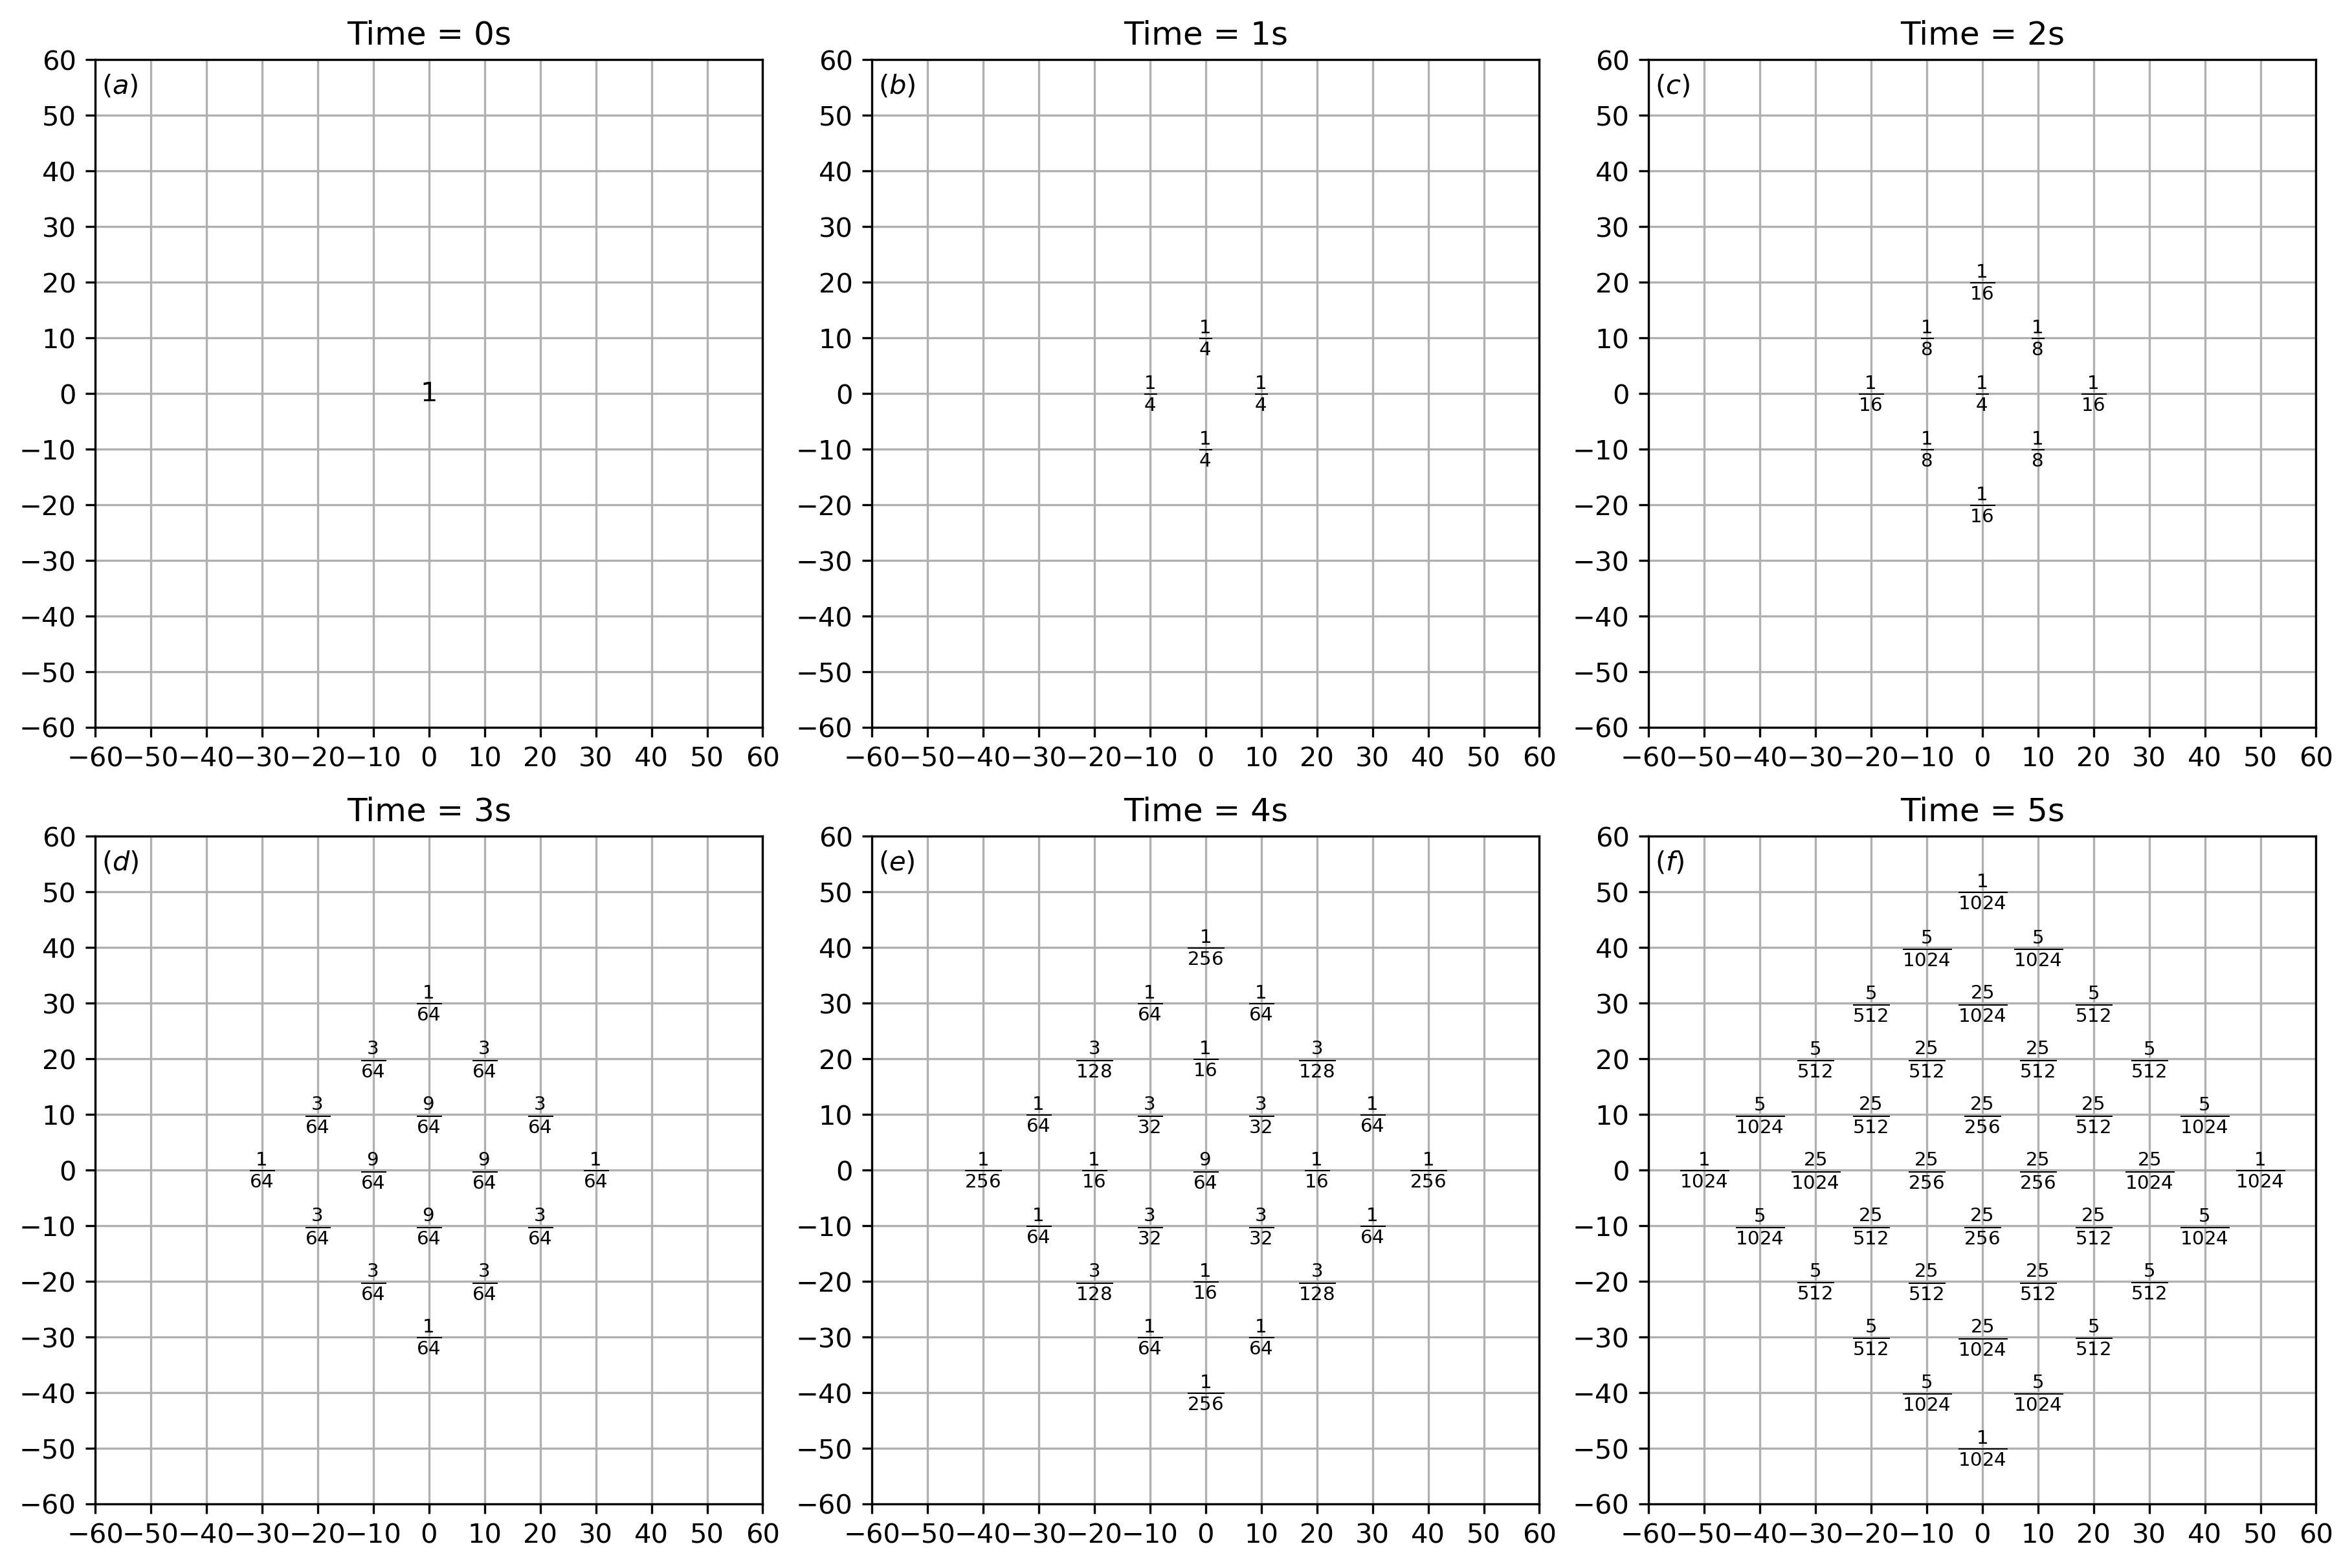
\includegraphics[width=\textwidth]{../Code/fig1.png}
    \caption{Figure showing the evolution of the spatial probability $\phi_{x,t}$ using snapshots from $t=0$ in (a) to $t=5$ in (f)}
    \label{fig1}
\end{figure}

One of the approaches to this problem is as follows. Let us assume that a large number of ants $a$ start from the origin. Every second, they randomly move \SI{10}{cm} directly north, south, east or west with equal probability. Therefore, this implies that after the first second, it is likely that $a/4$ ants end up at $(\SI{0}{cm}, \SI{10}{cm})$, $a/4$ ants at $(\SI{10}{cm}, \SI{0}{cm})$, $a/4$ ants at $(\SI{-10}{cm}, \SI{0}{cm})$, and $a/4$ ants at $(\SI{0}{cm}, \SI{-10}{cm})$ as shown in figure \ref{fig1}a. In each subsequent second, a quarter of ants at any given location will move to the north, a quarter to the south, a quarter to the east, and a quarter to the west. If ants from multiple locations converge on a single point, their numbers add up. Using this method, locations and number of ants are predictable at each subsequent second as shown in \ref{fig1}a-f. It can be seen that a pattern emerges while tracking the positions and numbers of the ants. 

\subsection{Average time for question 1}

\begin{figure}
    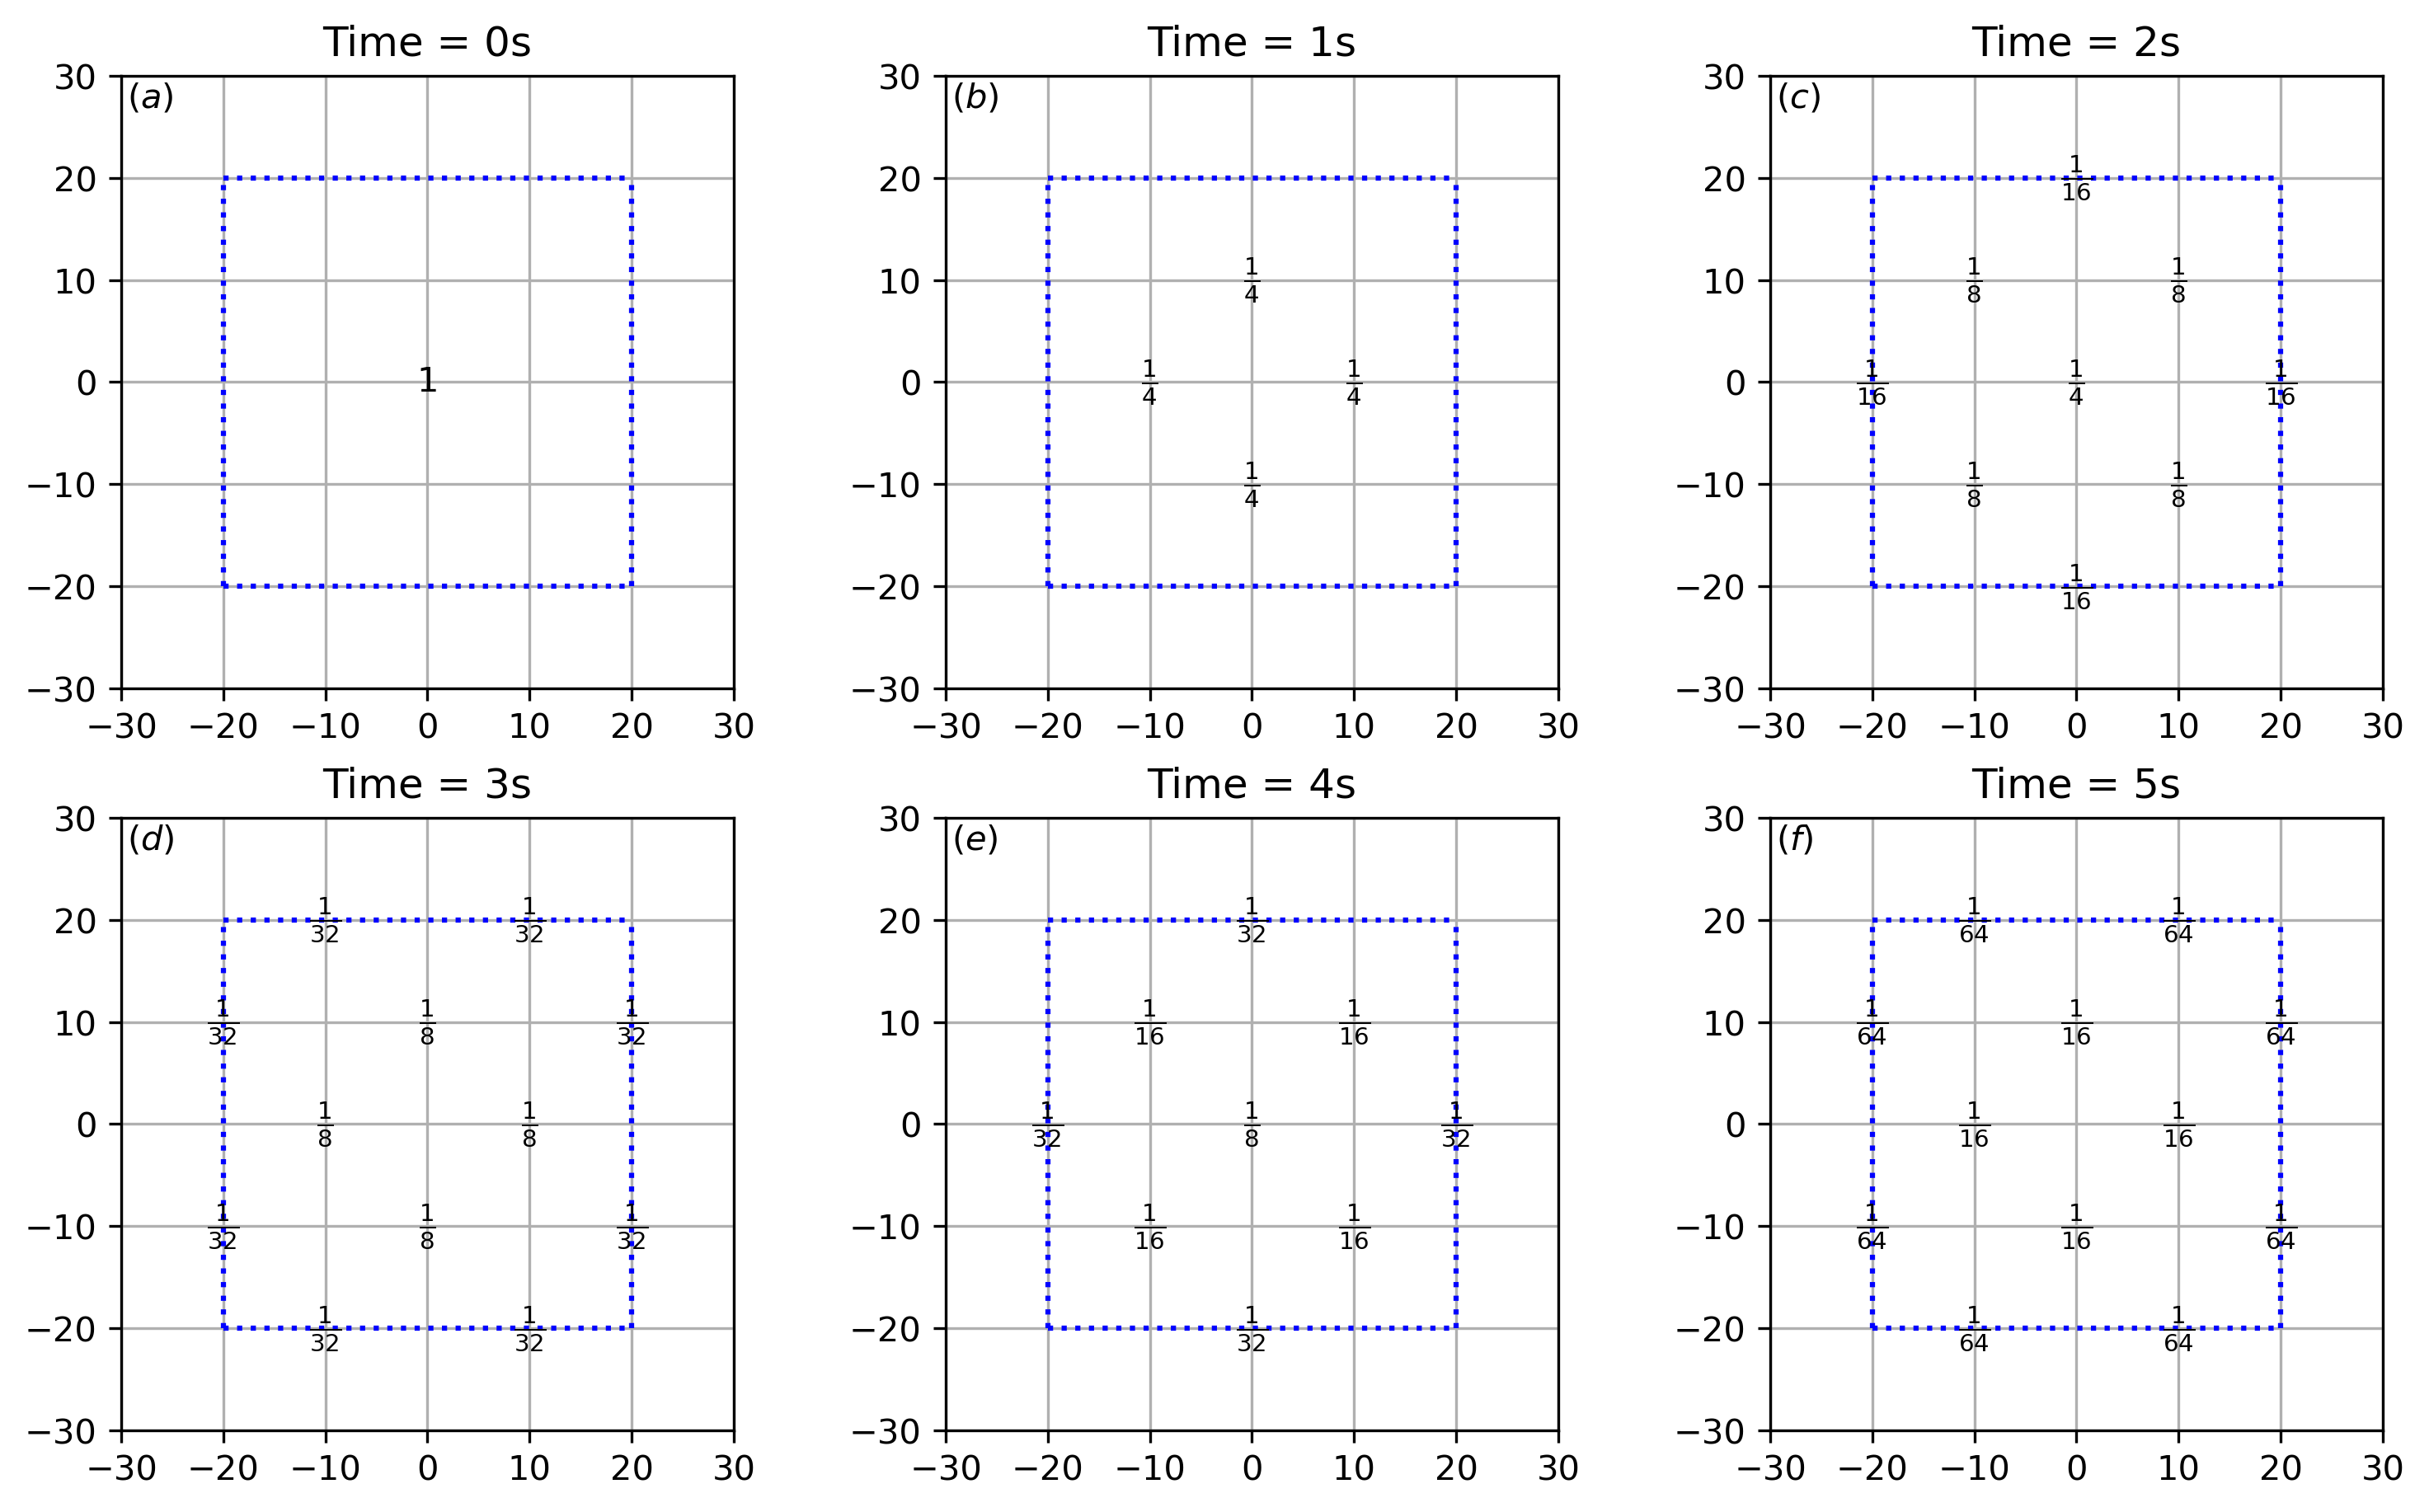
\includegraphics[width=\textwidth]{../Code/fig2.png}
    \caption{Figure showing the evolution of the spatial probability $\phi_{x,t}$ using snapshots from $t=0$ in (a) to $t=5$ in (f). The boundary where food is present is shown in blue. Once ants reach this boundary, they are no longer tracked as their spatial probability distribution no longer contributes to the average time.}
    \label{fig2}
\end{figure}

After \SI{2}{s}, the first ants reach the square boundary given by east-west lines \SI{20}{cm} to the north and \SI{20}{cm} to the south, as well as on north-south lines \SI{20}{cm} to the east and \SI{20}{cm} to the west from the anthill. We can then use the fraction of the number of ants $\phi_{t,b}$ that have reached the boundary at any given time $t$ to compute a weighted average that gives the average time $\overline{t}$ taken by all ants to reach the food. Therefore, we write 
\begin{equation}
    \overline{t} = \sum{t\phi_{t,b}}.
    \label{eqn1}
\end{equation}
From the pattern apparent in figures \ref{fig2}a-f, the value of $\phi_{t,b}$ can be predicted as
\begin{equation}
    \phi_{t,b} = 
    \begin{cases}
        0 & \text{if } t < 2\\
        \frac{4}{2^{t+2}} & \text{if } t \text{ is even}\\
        \frac{8}{2^{t+3}} & \text{if } t \text{ is odd}
    \end{cases}.
\end{equation}
Therefore, the weighted mean for the average time taken to reach the food using (\ref{eqn1}) can be written as an infinite sum as
\begin{equation}
    \overline{t} = 0 + 0 + 2(\frac{4}{16}) + 3(\frac{8}{32}) + 4(\frac{4}{32}) + 5(\frac{8}{64}) + 6(\frac{4}{64}) + ...,
\end{equation} 
which can also be written (after some simplification) as a general summation 
\begin{equation}
    \overline{t} = \sum_{n=1}^{\infty} \frac{4n+1}{2^{n+1}}.
\end{equation} 
This summation can be split into two parts for ease of computation as 
\begin{equation}
    \overline{t} = \sum_{n=1}^{\infty} \frac{1}{2^{n+1}} + \sum_{n=1}^{\infty} \frac{4n}{2^{n+1}}.
\end{equation} 
It is trivial to compute that the summation of the first term is $\frac{1}{2}$ given that it is a geometric series. The second term can be written as 
\begin{equation}
    \sum_{n=1}^{\infty} \frac{4n}{2^{n+1}} = \left.\left(\frac{\partial}{\partial \xi}\sum_{n=1}^{\infty} \left(\frac{\xi}{2}\right)^n\right)\right|_{x=1},
\end{equation}
which can be shown to be $4$ by taking the derivative of the formula for the sum of a geometric series evaluated at $\xi=1$. Therefore, the average time for ants to reach the food for this case is equal to \SI{4.5}{s}.

\begin{figure}
    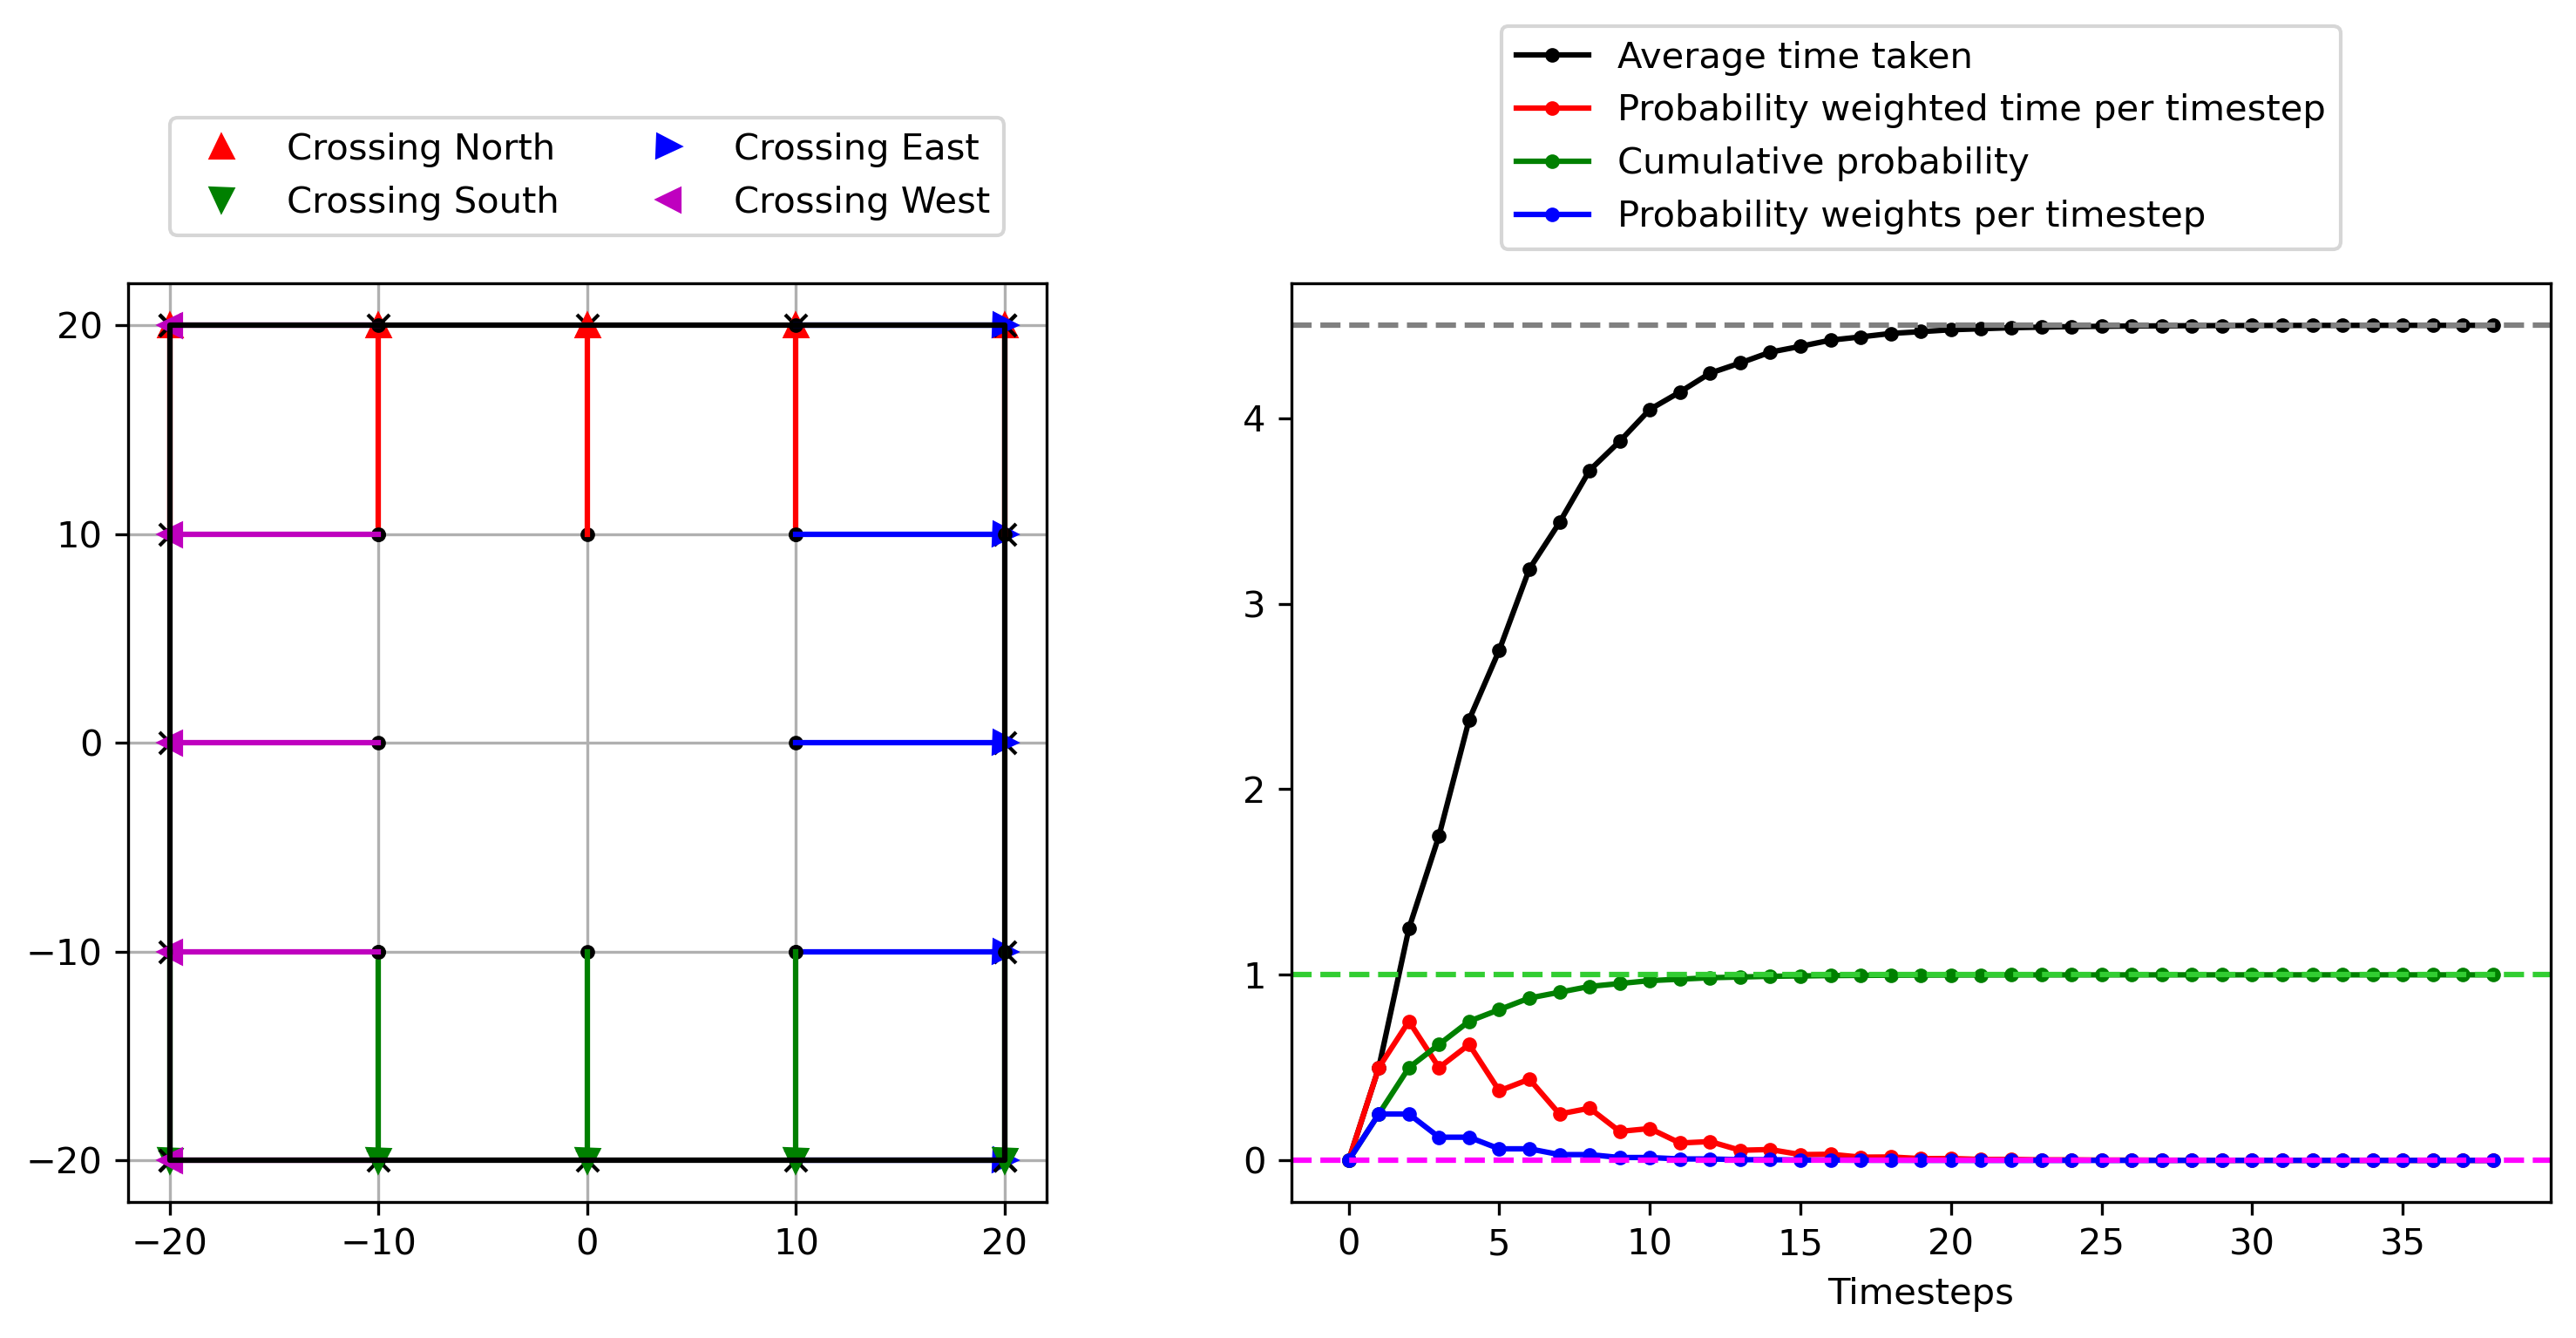
\includegraphics[width=\textwidth]{../Code/question1.png}
    \caption{Figure showing (a) the locations where ants cross the boundary and find food using triangular markers and (b) the plot showing the convergence of $\overline{t}$, $\phi_{b,t}$, $t\phi_{b,t}$, and cumulative probability of all ants crossing the boundary.}
    \label{que1}
\end{figure}

\subsection{Average time for question 2}

\begin{figure}
    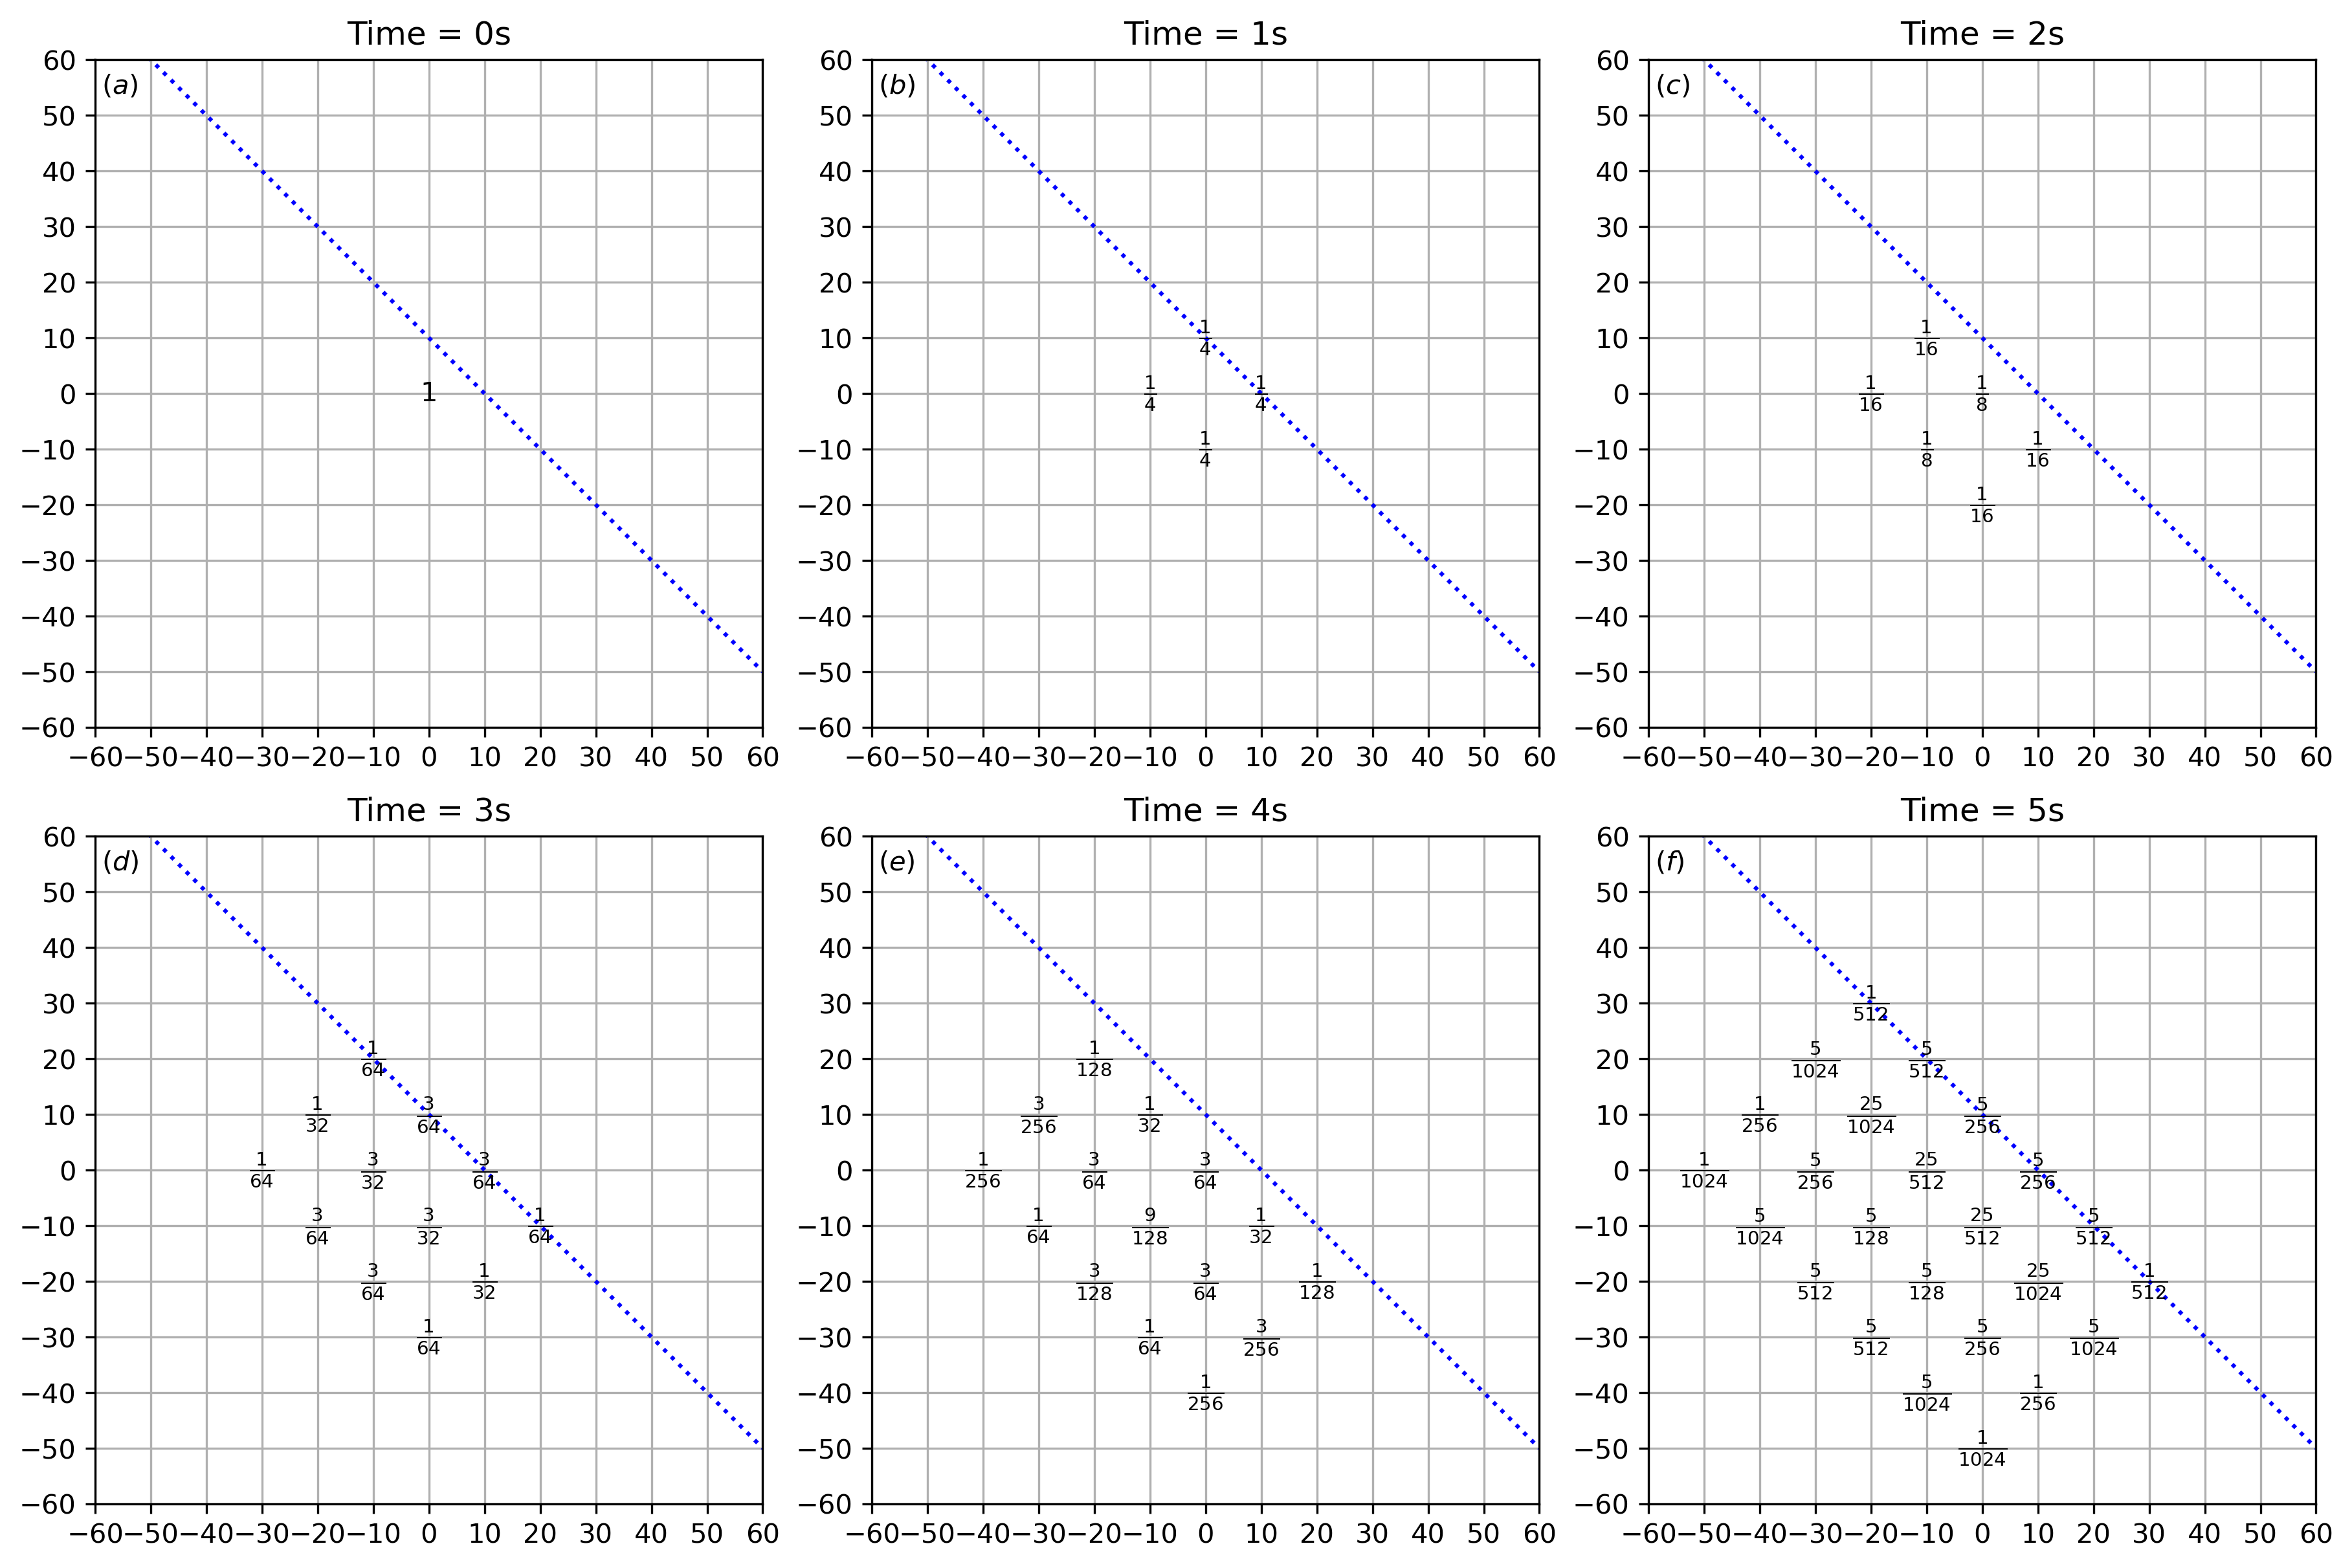
\includegraphics[width=\textwidth]{../Code/fig3.png}
    \caption{Figure showing the evolution of the spatial probability $\phi_{x,t}$ using snapshots from $t=\SI{0}{s}$ in (a) to $t=\SI{5}{s}$ in (f). The line where food is present is shown in blue. Once ants reach this line, they are no longer tracked as their spatial probability distribution no longer contributes to the average time.}
    \label{fig3}
\end{figure}

\begin{figure}
    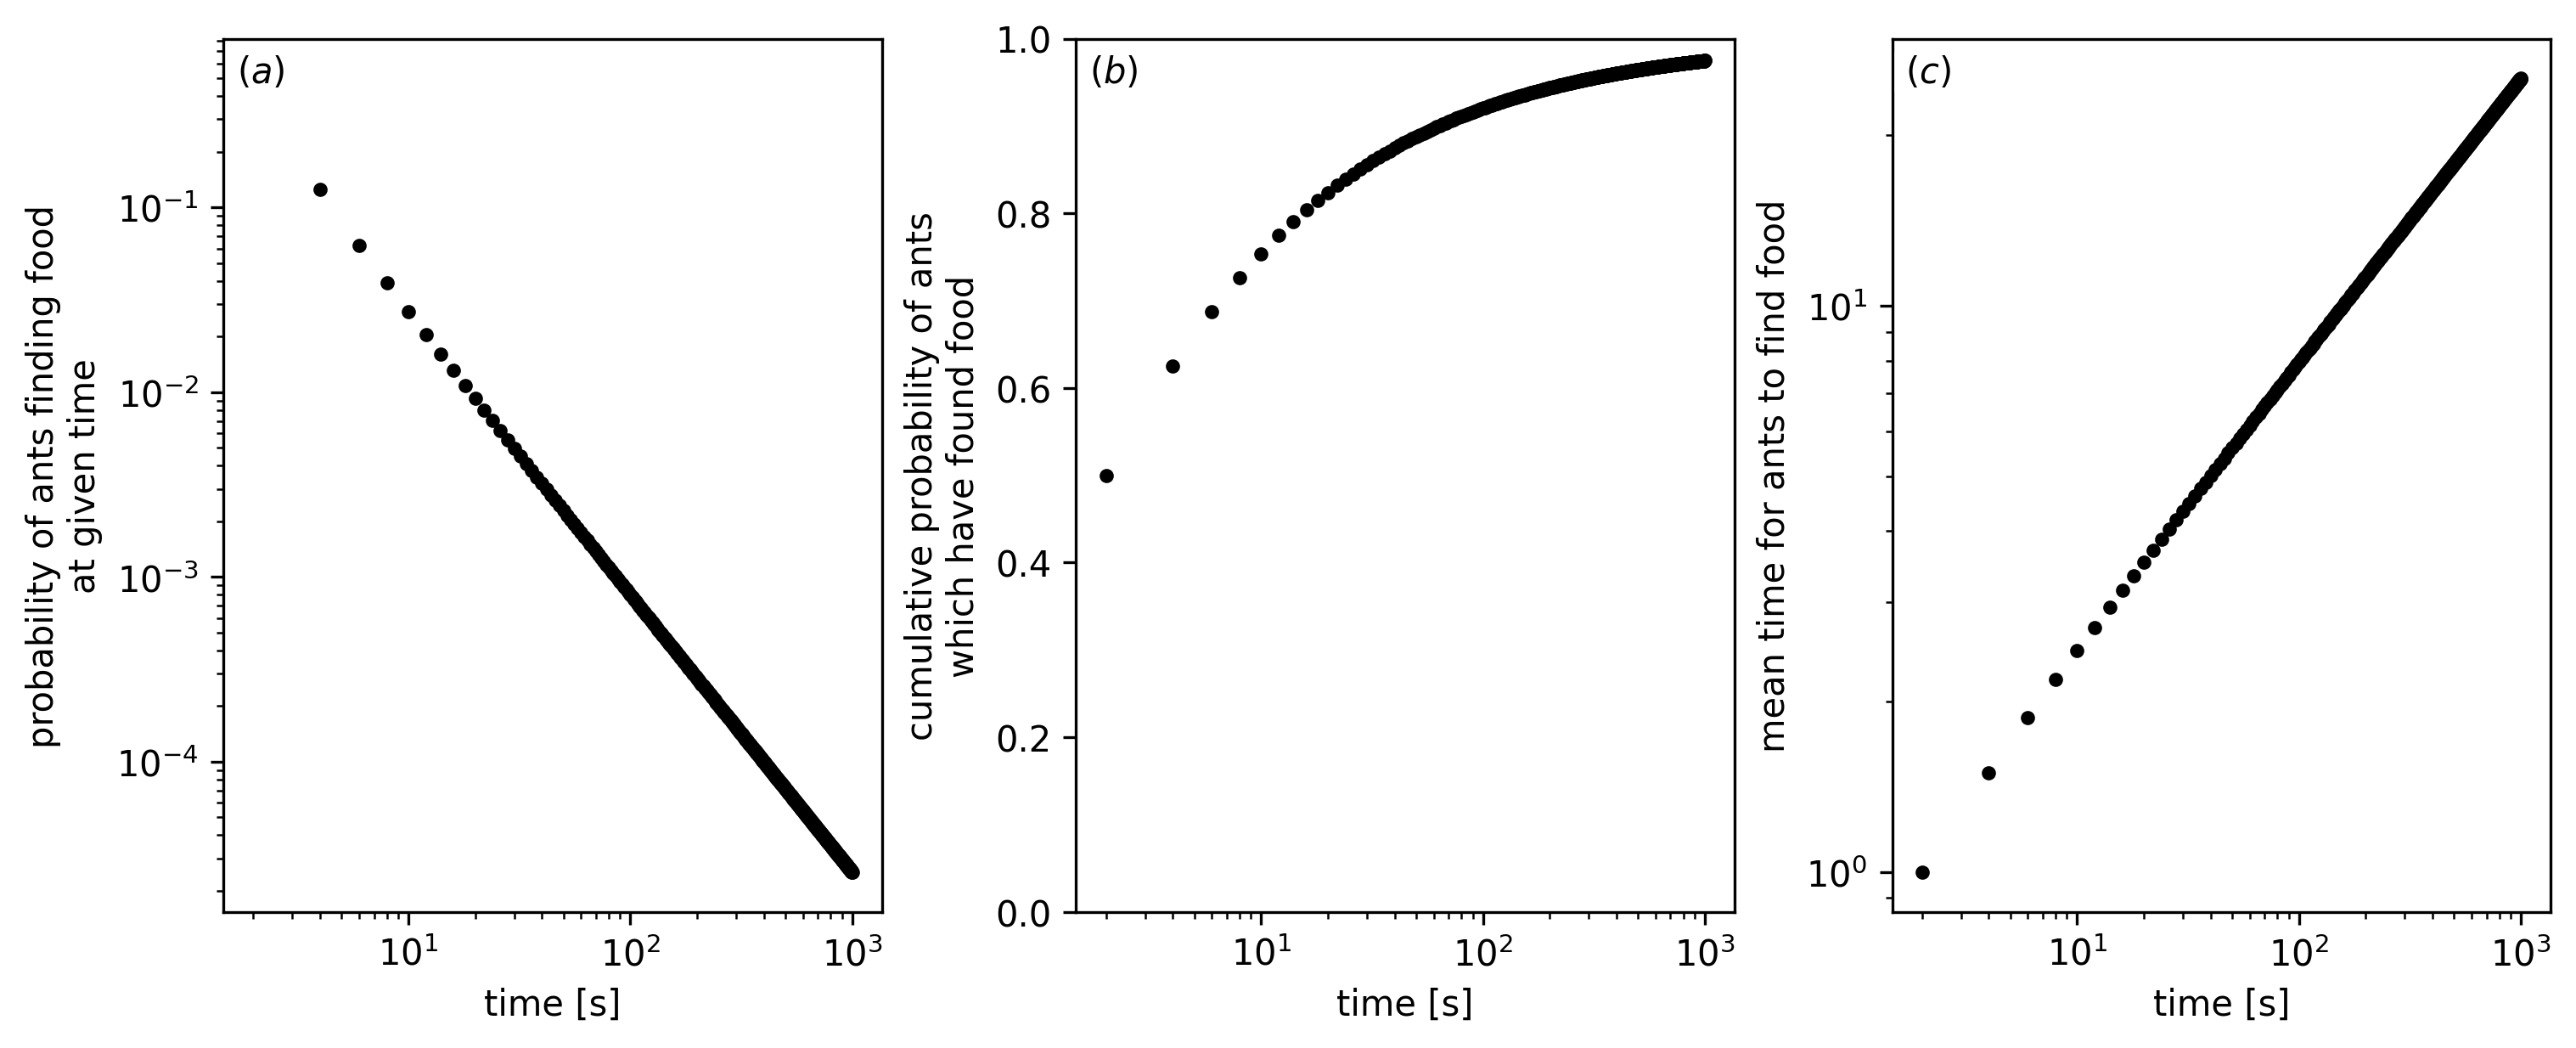
\includegraphics[width=\textwidth]{../Code/question2.png}
    \caption{Figure showing (a) the evolution of the probability $\phi_{b,t}$ as a function of time, (b) the cumulative probability of all ants that have found food as a function of time and (c) the mean time taken for ants $(\overline{t})$ as given by (\ref{eqn1}) computed as a function of time showing no convergence and an unbounded growth. Note that only points at odd integral time are plotted because $\phi_{b,t}$ is zero at even integral time.}
    \label{que2}
\end{figure}

A similar approach by studying the patter in figures \ref{fig3}a-f can be utilized to compute a weighted sum giving us the average time taken by ants to reach the line passing through points $(\SI{10}{cm}, \SI{0}{cm})$ and $(\SI{0}{cm}, \SI{10}{cm})$. However, computing this mean time $\phi_{t,b}$ shows us that it does not converge to any finite value, but instead continues to grow in an unbounded fashion as shown in \ref{que2}c. Therefore, the mean time for ants to reach food in this case is infinite. 

\subsection{Average time for question 3}

\begin{figure}
    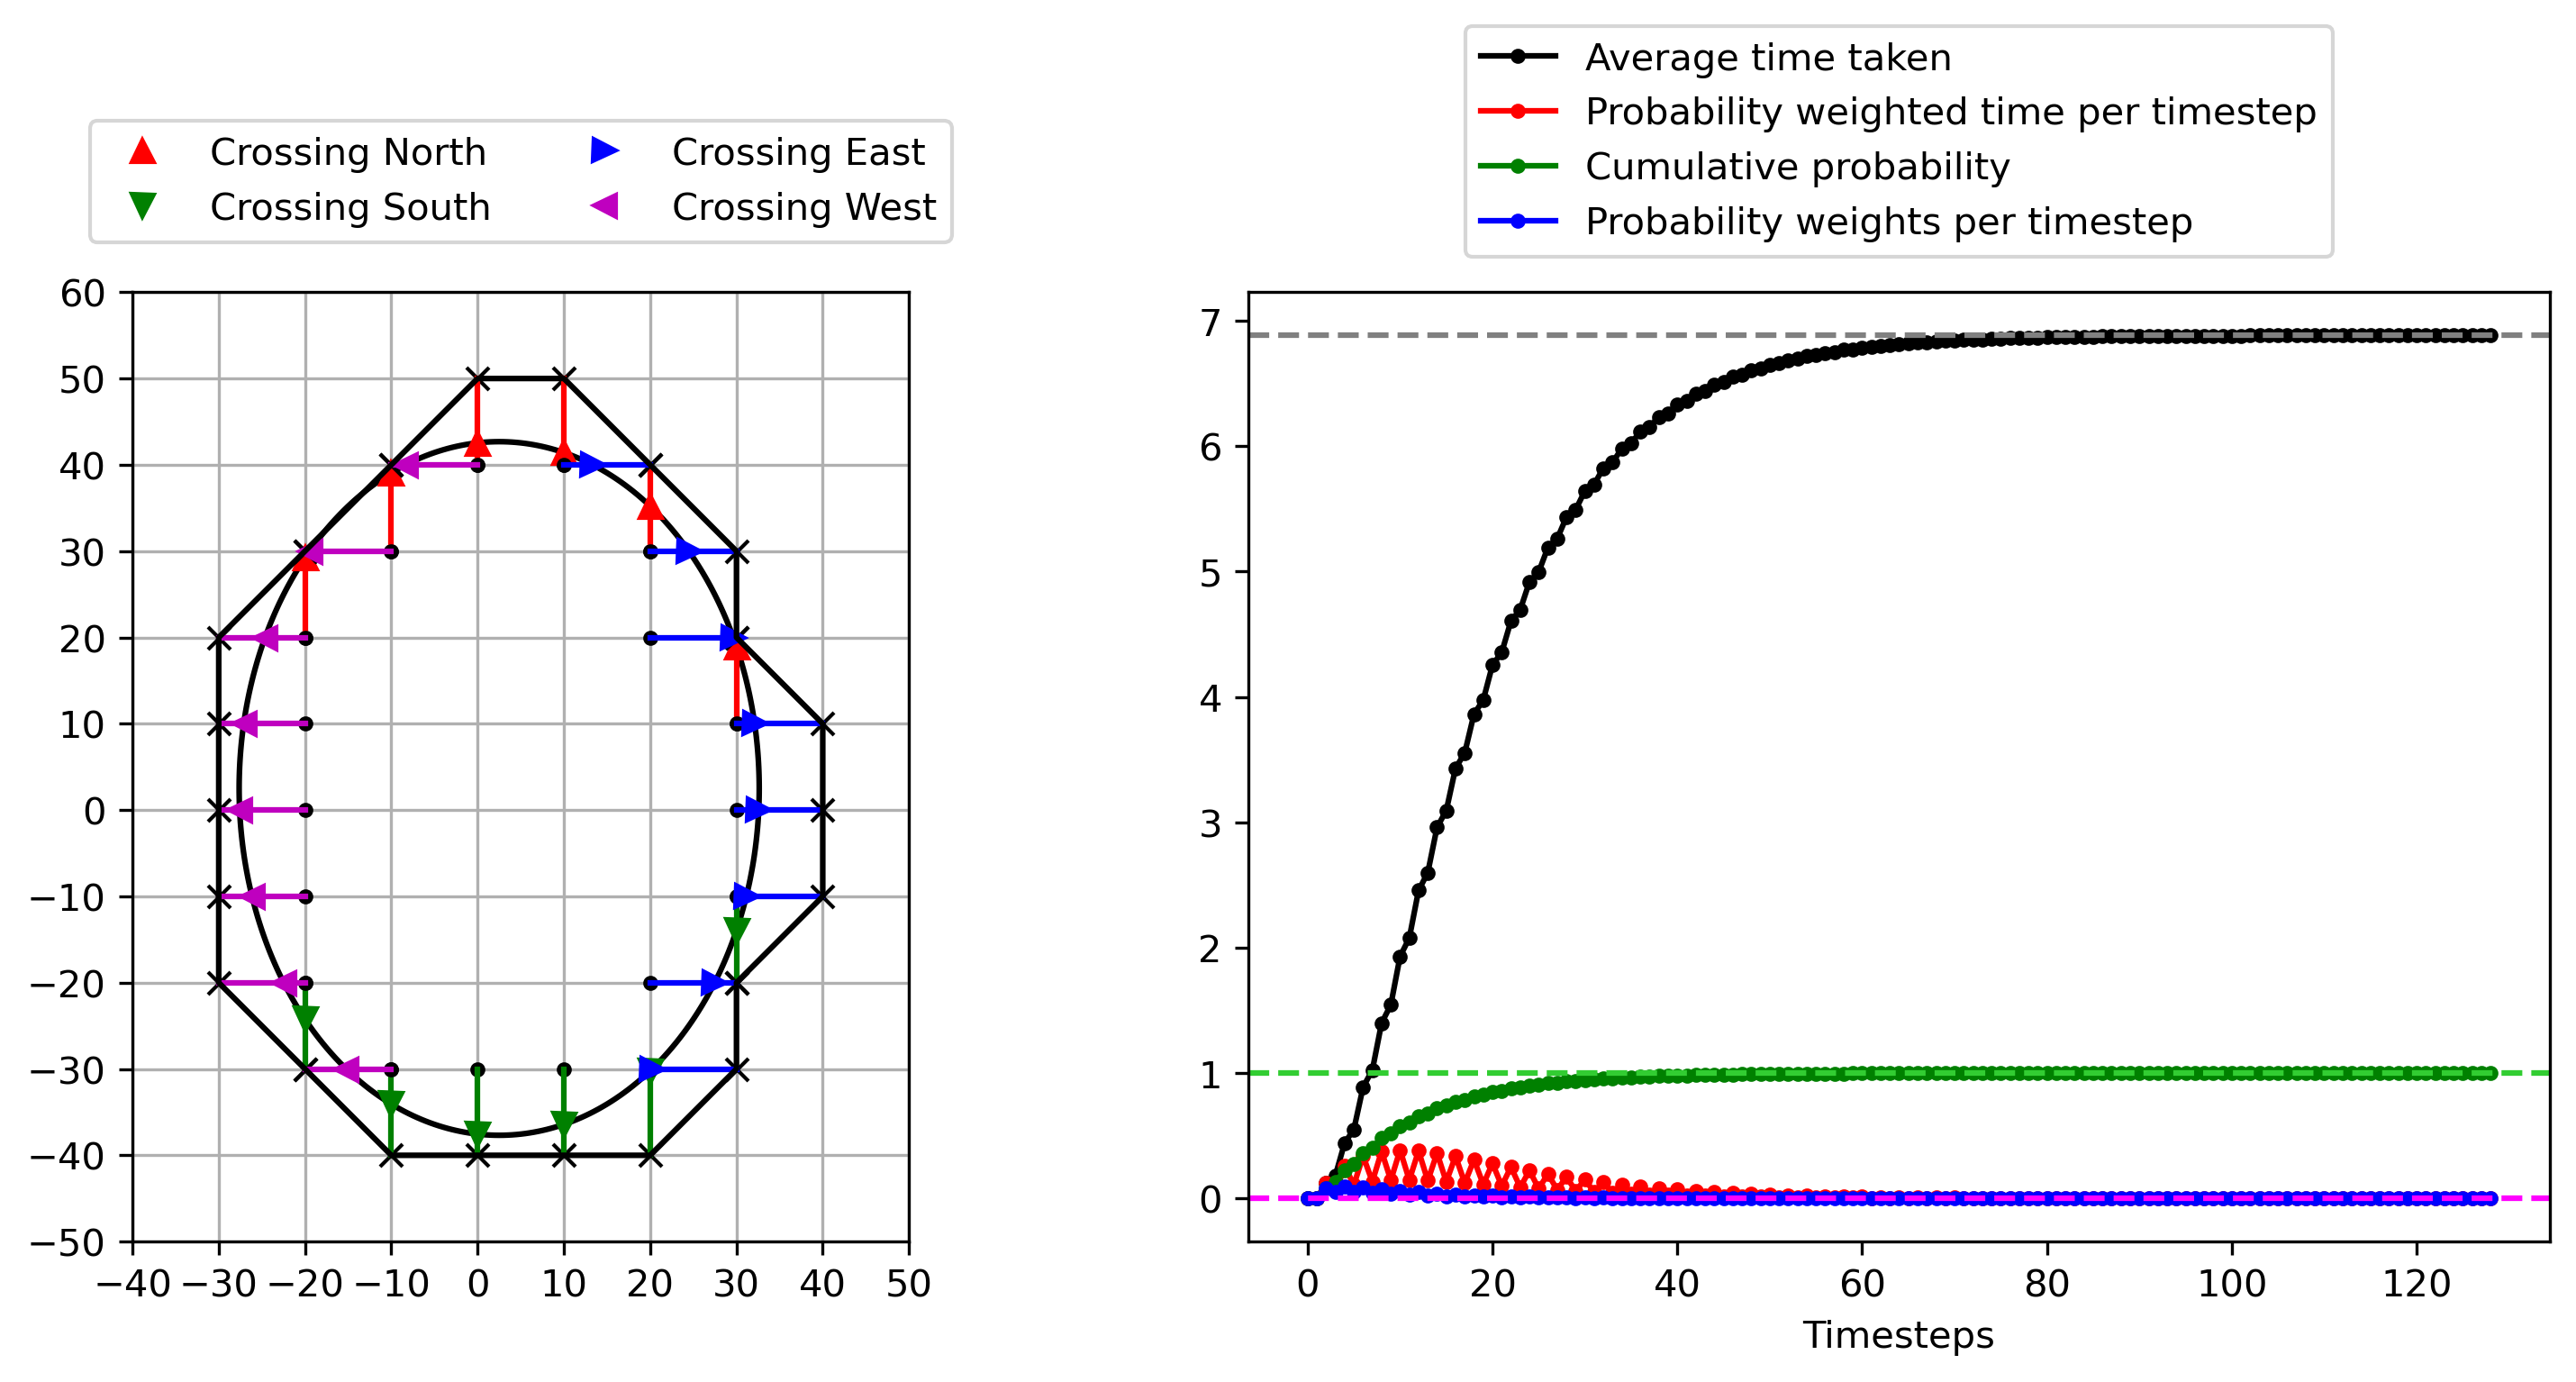
\includegraphics[width=\textwidth]{../Code/question3.png}
    \caption{Figure showing (a) the locations where ants cross the boundary and find food using triangular markers and (b) the plot showing the convergence of $\overline{t}$, $\phi_{b,t}$, $t\phi_{b,t}$, and cumulative probability of all ants crossing the boundary.}
    \label{que3}
\end{figure}

For the ellipse given by $\left( (x - \SI{2.5}{cm}) / \SI{30}{cm} \right)^2 + \left( (y - \SI{2.5}{cm}) / \SI{40}{cm} \right)^2 < 1$, a purely computational approach is used. Evolution of probability is tracked on a grid and ants crossing the boundary are removed. When the boundary does not conform to the integral grid given by the distance travelled by the ant in a second, the fractional time taken to reach food is accounted for by finding the intersection with the polynomial curve as shown in figure \ref{que3}a. The convergence of the average time taken by ants is shown in figure \ref{que3}b and the mean value is $\approx \SI{6.88}{s}$.

\end{document}